% =========================================================================
% SECCIONES PARA EL TRABAJO DE FIN DE GRADO (TFG)
% Título sugerido: Clasificación Automática de Lesiones de LCA mediante 
%                 Modelos de Aprendizaje Profundo Basados en Vision Transformers
% Autor: Palodo2 - Universidad de Valencia
% =========================================================================

% -------------------------------------------------------------------------
% SECCIÓN 1: DATOS DEL ESTUDIO
% -------------------------------------------------------------------------
\section{Datos del estudio}
\label{sec:datos_estudio}

El presente estudio se centra en el desarrollo y evaluación de modelos de aprendizaje profundo para la clasificación automática de lesiones del ligamento cruzado anterior (LCA) a partir de volúmenes de resonancia magnética (RM) de rodilla. El conjunto de datos principal utilizado en este trabajo está derivado del dataset de referencia pública \textbf{MRNet}, desarrollado por la Escuela de Medicina de la Universidad de Stanford. Con el fin de evaluar la robustez y capacidad de generalización del sistema en un entorno clínico real, se ha incorporado un conjunto de datos de validación externa independiente procedente de una cohorte clínica de Croacia (\textit{Croatia Dataset}).


\subsection{Cohortes de Pacientes y Particiones del Dataset}
Para garantizar la fiabilidad del entrenamiento y evitar el sesgo de información o fuga de datos (\textit{data leakage}), el conjunto de datos de Stanford (MRNet) se dividió a nivel de paciente en tres subconjuntos mutuamente excluyentes: entrenamiento (\textit{Train}), validación (\textit{Validation}) y prueba interna (\textit{Test}). El conjunto de validación externa (cohorte de Croacia) se mantuvo completamente aislado y solo se utilizó para la evaluación final de generalización.

Es importante destacar que el conjunto de datos clínicos original presenta un marcado desbalance de clases, lo cual es altamente representativo de la práctica clínica radiológica real, donde la prevalencia de roturas de LCA es sustancialmente menor que la de estudios normales o con otras patologías de rodilla. La prevalencia global de lesiones de LCA en los datos internos de Stanford es del $20.96\%$ (262 casos positivos frente a 988 controles de un total de 1250 estudios), lo cual exige el uso de regularizaciones robustas y métricas de evaluación independientes del balance de clases, como el F1-Score y el AUC-ROC, para evitar que los clasificadores se sesguen hacia la clase mayoritaria.

La distribución exacta de los casos clínicos y el balance de clases en cada partición se detallan en la Tabla~\ref{tab:distribucion_datos}.

\begin{table}[htbp]
\centering
\caption{Distribución de los conjuntos de datos, número de muestras y prevalencia real de la lesión de LCA.}
\label{tab:distribucion_datos}
\begin{tabular}{lccccc}
\hline
\textbf{Conjunto de Datos} & \textbf{Casos Totales} & \textbf{LCA Lesionado (+)} & \textbf{Control (-)} & \textbf{Prevalencia (\%)} & \textbf{Propósito Clínico} \\ \hline
Entrenamiento (Train)      & 875                    & 183                        & 692                  & 20.91\%                    & Ajuste de parámetros \\
Validación (Validation)    & 188                    & 36                         & 152                  & 19.15\%                    & Optimización de hiperparámetros \\
Prueba Interna (Test)      & 187                    & 43                         & 144                  & 22.99\%                    & Evaluación del rendimiento \\
Validación Externa (Croacia)& 145                    & 67                         & 78                   & 46.21\%                    & Prueba de generalización \\ \hline
\textbf{Total Global}      & \textbf{1395}          & \textbf{329}               & \textbf{1066}        & \textbf{23.58\%}           & -- \\ \hline
\end{tabular}
\end{table}


\subsection{Estructura y Representación de los Datos de RM}
Cada estudio de resonancia magnética consta de tres series tridimensionales correspondientes a los tres planos anatómicos estándar:
\begin{enumerate}
    \item \textbf{Plano Sagital}: Fundamental para evaluar la continuidad de las fibras del LCA y detectar signos indirectos como la traslación tibial anterior.
    \item \textbf{Plano Coronal}: Útil para verificar la inserción femoral y tibial del ligamento.
    \item \textbf{Plano Axial}: Permite observar el LCA en su trayecto a través de la fosa intercondílea.
\end{enumerate}

Matemáticamente, cada volumen tridimensional de RM se representa como un tensor $V \in \mathbb{R}^{S \times H \times W}$, donde $S$ es el número variable de cortes (\textit{slices}) en la serie, $H$ es la altura del corte y $W$ es la anchura. En el conjunto de datos crudo, cada corte posee una resolución espacial de $256 \times 256$ píxeles con una profundidad de bits en escala de grises. 

Durante la etapa de carga de datos, implementada en la clase customizada \texttt{OptimizedMRNetDataset} (ver Listing~\ref{lst:dataloader}), los datos se preprocesan dinámicamente:
\begin{equation}
    x_{\text{norm}} = \frac{x - x_{\text{min}}}{x_{\text{max}} - x_{\text{min}}}
\end{equation}
donde $x$ representa los valores de intensidad de píxel originales de los cortes seleccionados. Este proceso de normalización Min-Max escala las intensidades al rango $[0, 1]$, homogeneizando las variaciones de contraste producidas por distintos escáneres de RM. Posteriormente, los tensores se interpolan a una dimensión de $224 \times 224$ píxeles y se replican a lo largo de 3 canales (simulando una imagen RGB) para permitir la inicialización con pesos pre-entrenados de arquitecturas basadas en ImageNet.

\begin{lstlisting}[language=Python, caption={Detalle de la implementación de carga de datos en PyTorch mostrando la normalización Min-Max y la replicación a 3 canales.}, label=lst:dataloader, frame=single, basicstyle=\ttfamily\small]
# Fragmento extraído de src/data_loader.py
# Normalización Min-Max del volumen seleccionado
vol_min = selected_slices.min()
vol_max = selected_slices.max()
if vol_max > vol_min:
    selected_slices = (selected_slices - vol_min) / (vol_max - vol_min)

# Conversión a tensor y replicación a 3 canales para compatibilidad con ViT
selected_slices = torch.from_numpy(selected_slices).float()
selected_slices = selected_slices.unsqueeze(1)  # (K, 1, H, W)
selected_slices = selected_slices.repeat(1, 3, 1, 1)  # (K, 3, H, W)
\end{lstlisting}

% -------------------------------------------------------------------------
% SECCIÓN 2: DISEÑO EXPERIMENTAL
% -------------------------------------------------------------------------
\section{Diseño experimental}
\label{sec:diseno_experimental}

El diseño experimental de este TFG plantea un enfoque de ensamble multi-vista e independiente por plano anatómico. Debido a las marcadas diferencias morfológicas y clínicas de la representación del ligamento cruzado anterior en cada plano, entrenar un único modelo tridimensional global suele sufrir de sobreajuste (\textit{overfitting}) debido al limitado tamaño muestral. Por tanto, se opta por entrenar tres clasificadores especializados (uno por plano) cuyas predicciones probabilísticas finales se combinan mediante una estrategia de ensamble de votación ponderada.

\subsection{Definición del Flujo del Sistema}
El flujo general de predicción del sistema sigue el esquema estructurado en la Figura~\ref{fig:flujo_mri}:
\begin{enumerate}
    \item \textbf{Entrada}: Un volumen 3D de RM compuesto por sus tres planos.
    \item \textbf{Extracción Estratégica de Cortes}: Selección de los $K$ cortes más significativos por plano clínico.
    \item \textbf{Clasificación de Redes de Aprendizaje Profundo}: Procesamiento en paralelo mediante modelos avanzados de redes convolucionales (CNN) o Vision Transformers (ViT).
    \item \textbf{Agregación Temporal/Espacial}: Fusión de las características de los $K$ cortes mediante \textit{Attention Pooling}.
    \item \textbf{Fusión del Ensamble}: Combinación de las probabilidades de salida de los tres planos mediante pesos optimizados.
    \item \textbf{Salida}: Clasificación binaria (Lesión de LCA: SÍ/NO) junto con el nivel de confianza del modelo.
\end{enumerate}

\begin{figure}[htbp]
\centering
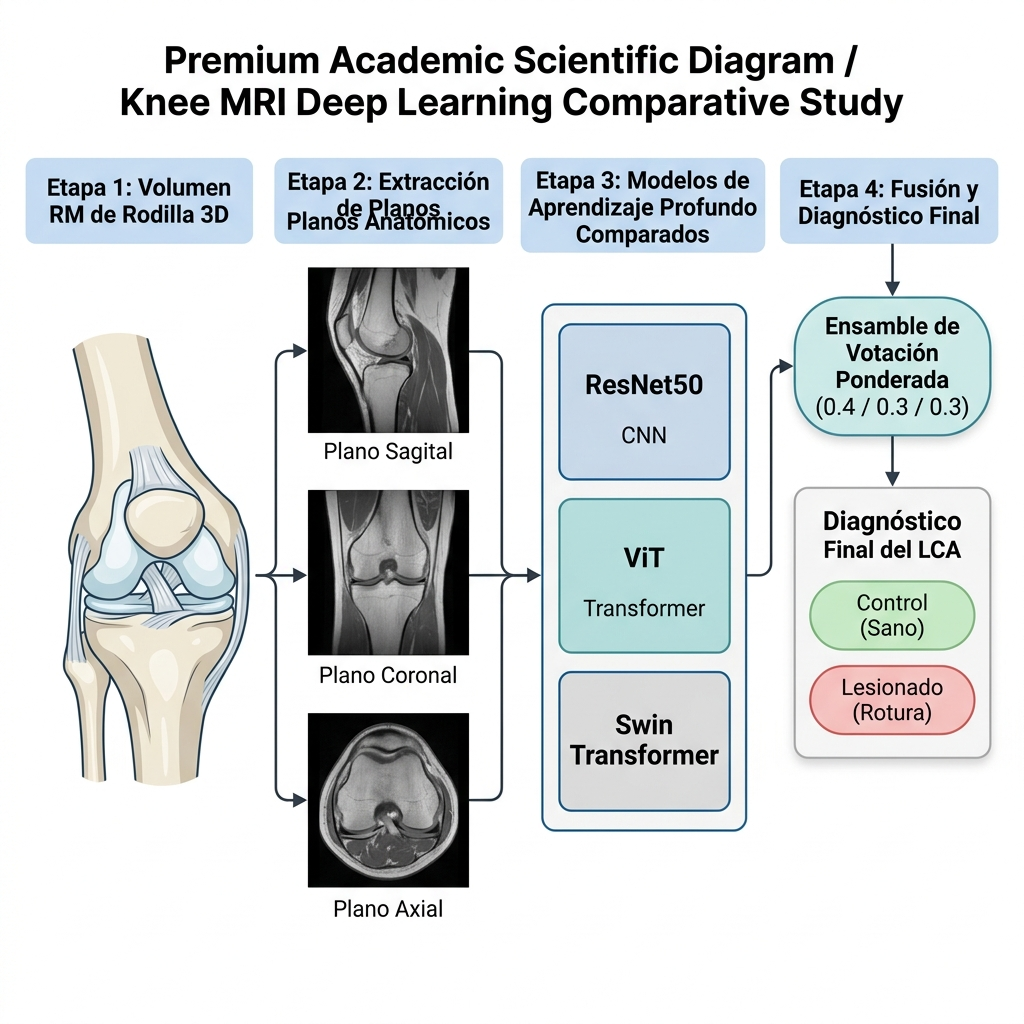
\includegraphics[width=0.85\textwidth]{figuras/mri_ensemble_pipeline.png}
\caption{Flujo metodológico detallado del ensamble multi-plano propuesto. Muestra el procesamiento paralelo de los planos sagital, coronal y axial mediante clasificadores de aprendizaje profundo independientes (CNNs o Transformers) y su fusión final por votación ponderada.}
\label{fig:flujo_mri}
\end{figure}

\subsection{Selección de Cortes Anatómicos (Estrategias de Slicing)}
Procesar la totalidad de los cortes de un volumen de RM clínico (que suele oscilar entre 20 y 45 cortes) introduce un excesivo ruido de fondo e incrementa innecesariamente el coste computacional, dado que el ligamento solo es visible en una ventana espacial limitada. Se han diseñado y comparado tres estrategias para extraer una secuencia fija de $K$ cortes significativos:
\begin{itemize}
    \item \textbf{Estrategia Center}: Consiste en extraer los $K$ cortes centrales del volumen basándose puramente en la indexación geométrica de la serie.
    \item \textbf{Estrategia CNN-Based (Recomendación)}: Utiliza una red convolucional ligera pre-entrenada para evaluar la presencia del LCA en cada corte, seleccionando una ventana consecutiva de $K$ cortes con las mayores puntuaciones de confianza.
    \item \textbf{Estrategia Random} (utilizada exclusivamente durante el entrenamiento): Introduce perturbaciones aleatorias desplazando el centro de la ventana de selección de cortes para actuar como regularizador de aumento de datos.
\end{itemize}

De acuerdo con el análisis empírico, la configuración óptima establecida para el pipeline es:
\begin{itemize}
    \item \textbf{Sagital}: $K=5$ cortes seleccionados mediante \textit{CNN-Based}.
    \item \textbf{Coronal}: $K=10$ cortes seleccionados mediante \textit{CNN-Based}.
    \item \textbf{Axial}: $K=10$ cortes seleccionados mediante \textit{Center Consecutive}.
\end{itemize}
\subsection{Modelos de Aprendizaje Profundo Comparados: Convoluciones y Transformers}
Para este estudio comparativo se han seleccionado y evaluado cinco arquitecturas de red altamente representativas de los dos paradigmas dominantes en visión por computador: las Redes Convolucionales (CNN) y los Vision Transformers (ViT), adaptando sus capacidades al análisis volumétrico de rodilla.

Las arquitecturas entrenadas y analizadas en este estudio comparativo son:
\begin{itemize}
    \item \textbf{CNN-ResNet50}: Red convolucional profunda clásica basada en bloques residuales (23.5M parámetros), utilizada como la línea base de referencia médica tradicional.
    \item \textbf{ConvNeXt V2 Tiny}: Un modelo convolucional de última generación (28.6M parámetros) que moderniza el diseño CNN incorporando filosofías de los Transformers (como kernels de convolución grandes y activaciones GeLU).
    \item \textbf{ViT-Small}: El Vision Transformer estándar en su escala pequeña (22.0M parámetros), que modela dependencias espaciales globales dividiendo cada corte en parches de $16\times16$ píxeles.
    \item \textbf{ViT-Tiny}: La versión ultra-compacta del Vision Transformer estándar (5.7M parámetros), útil para analizar el impacto clínico de reducir drásticamente la capacidad de parámetros.
    \item \textbf{Swin-Small}: Vision Transformer jerárquico de escala pequeña (49.7M parámetros) que calcula auto-atención sobre ventanas locales desplazadas de forma no solapada.
\end{itemize}

Las especificaciones técnicas y los rendimientos comparativos reales obtenidos por cada arquitectura en tu dataset se detallan en la Tabla~\ref{tab:arquitecturas}.

\begin{table}[htbp]
\centering
\caption{Comparativa real de parámetros y rendimiento diagnóstico (AUC-ROC) de lesiones de LCA en las particiones de validación y prueba.}
\label{tab:arquitecturas}
\begin{tabular}{lccccc}
\hline
\textbf{Modelo} & \textbf{Familia de Red} & \textbf{Parámetros} & \textbf{AUC Val} & \textbf{AUC Test} & \textbf{Threshold Óptimo} \\ \hline
\textbf{CNN-ResNet50}      & Convolucional Clásica  & 23.5 M              & \textbf{0.9879}  & \textbf{0.9432}   & 0.570 \\
\textbf{Swin-Small}        & Transformer Jerárquico & 49.7 M              & 0.9671           & 0.9356            & 0.580 \\
\textbf{ViT-Tiny}          & Transformer Estándar   & 5.7 M               & 0.9468           & 0.9309            & 0.410 \\
\textbf{ViT-Small}         & Transformer Estándar   & 22.0 M              & 0.9572           & 0.9278            & 0.550 \\
\textbf{ConvNeXt V2 Tiny}  & Convolucional Moderna  & 28.6 M              & 0.9790           & 0.9251            & 0.810 \\ \hline
\end{tabular}
\end{table}

\textit{Análisis Comparativo del Rendimiento}: Los resultados reales demuestran dinámicas científicas sumamente interesantes. La arquitectura clásica \textbf{CNN-ResNet50} obtuvo la puntuación de validación más alta del estudio (**0.9879 AUC**) y una excelente generalización en test (**0.9432 AUC**). Este comportamiento ratifica que las redes convolucionales, gracias a sus fuertes sesgos inductivos de invarianza a la traslación y localidad espacial, son sumamente robustas y eficientes cuando se entrenan con conjuntos de datos médicos de escala moderada, evitando el sobreajuste.

Por otro lado, la arquitectura Transformer jerárquica \textbf{Swin-Small} demostró una sólida capacidad de generalización en datos no vistos, alcanzando el **0.9356 AUC** en prueba. Esto demuestra la idoneidad de los mecanismos de atención por ventanas locales para capturar anomalías anatómicas sin incurrir en un sobreajuste severo en cohortes clínicas de tamaño moderado. En contraposición, los Transformers estándar (\textbf{ViT-Small} y \textbf{ViT-Tiny}), al carecer de estos sesgos inductivos de localidad y escala, obtienen resultados competitivos pero ligeramente inferiores en test (0.9278 y 0.9309 AUC). Finalmente, el modelo convolucional modernizado \textbf{ConvNeXt V2 Tiny} ofrece una robusta validación (0.9790 AUC) y un test de 0.9251.

\subsubsection{Vision Transformer Estándar (ViT-Base)}
El modelo \textit{Vision Transformer Base} (ViT-Base) \cite{dosovitskiy2020image} representa un cambio de paradigma en visión médica, al sustituir por completo los operadores convolucionales tradicionales por mecanismos de auto-atención global no local. 

Para su aplicación en cortes individuales de resonancia magnética de rodilla, la imagen de entrada en escala de grises $x \in \mathbb{R}^{H \times W \times C}$ (con $H=W=256$ y $C=3$) se divide inicialmente en parches bidimensionales no solapados $x_p \in \mathbb{R}^{N \times (P^2 \cdot C)}$, donde $P=16$ es la resolución del parche espacial y $N = (H \cdot W) / P^2 = 256$ es la secuencia de longitud del vector resultante. Cada parche se proyecta linealmente a un espacio vectorial de características de dimensión $D = 768$ y se concatena con un vector de \textit{embedding} de clase indexado (\textit{class token}) $x_{\text{class}} \in \mathbb{R}^{D}$. Adicionalmente, se añade un operador posicional sumatorio unidimensional apriorístico $E_{\text{pos}} \in \mathbb{R}^{(N+1) \times D}$ para preservar el orden espacial:
\begin{equation}
    z_0 = [x_{\text{class}}; x_p^1 E; x_p^2 E; \dots; x_p^N E] + E_{\text{pos}}
\end{equation}
El vector combinado se procesa secuencialmente a través de $L=12$ bloques Transformer idénticos. Cada bloque consta de una capa de Auto-Atención Multi-Cabeza (\textit{Multi-Head Self-Attention}, MHSA) y un Perceptrón Multicapa (\textit{Multi-Layer Perceptron}, MLP) con dos capas densas y activaciones GELU. El mecanismo de atención global se rige por el cálculo de consultas ($Q$), claves ($K$) y valores ($V$) a partir del escalado del producto escalar de las matrices proyectadas:
\begin{equation}
    \text{Attention}(Q, K, V) = \text{softmax}\left(\frac{Q K^T}{\sqrt{d_k}}\right) V
\end{equation}
donde $d_k$ denota la dimensión de escala de las cabezas de atención ($d_k = D / 12 = 64$). 

El entrenamiento de ViT-Base requirió un ajuste fino de regularización en el plano sagital debido a su baja tolerancia inherente al sobreajuste sobre muestras pequeñas. Se implementó una tasa de aprendizaje inicial de $1.3 \times 10^{-4}$ optimizada con AdamW, un decaimiento de peso (\textit{weight decay}) robusto de $1.5 \times 10^{-3}$, un factor de abandono de entrada (\textit{dropout input}) de $0.42$, y un factor de abandono interno en cabezas densas (\textit{dropout dense}) de $0.32$, estabilizado mediante un suavizado de etiquetas (\textit{label smoothing}) de $0.17$.

\subsubsection{Red Convolucional Residual de Línea Base (CNN-ResNet50)}
Como contraparte del paradigma convolucional clásico, se seleccionó el modelo \textit{ResNet50} \cite{he2016deep}, basado en bloques de aprendizaje residual. Su sesgo inductivo está intrínsecamente dotado de invarianza a la traslación y localidad espacial mediante el uso de filtros convolucionales pequeños ($3\times3$) de pesos compartidos distribuidos.

La formulación matemática de un bloque residual básico evita el desvanecimiento del gradiente en capas profundas mediante conexiones de atajo (\textit{skip connections}) que añaden la identidad de la señal de entrada $x$ directamente a la salida de las transformaciones no lineales $\mathcal{F}(x)$:
\begin{equation}
    y = \mathcal{F}(x, \{W_i\}) + W_s x
\end{equation}
donde $W_s$ representa una matriz de proyección lineal utilizada únicamente en caso de discrepancia de dimensiones de canal. 

La extracción volumétrica de características en ResNet50 genera un vector latente final de dimensión $D = 2048$ para cada corte, el cual se proyecta de forma homóloga al clasificador multietapa. El entrenamiento se optimizó bajo una arquitectura de alta tasa de regularización específica para mitigar el sobreajuste del \textit{backbone}:
\begin{itemize}
    \item \textbf{Sagital y Axial}: Optimizador AdamW con tasa de aprendizaje de $1.3 \times 10^{-4}$, regularizado con \textit{dropout} agresivo de $0.42$ en la fase de entrada del clasificador lineal y $0.32$ en las capas densas profundas, y decaimiento de pesos de $1.5 \times 10^{-3}$.
    \item \textbf{Coronal}: Se elevó el \textit{dropout input} a un valor extremo de $0.47$ acompañado de un suavizado de etiquetas de $0.22$ y una paciencia de parada temprana extendida a 30 épocas para estabilizar la lenta convergencia en el plano con mayor oclusión del LCA.
\end{itemize}

\section{Swin Transformers}

\subsection{Swin-Small}
\label{subsec:swin_small}

El modelo \textit{Shifted Window Transformer Small} (Swin-Small) \cite{liu2021swin} representa una evolución jerárquica de los Vision Transformers basada en mecanismos de atención local mediante ventanas desplazadas (\textit{Shifted Window Self-Attention}).

A diferencia de Vision Transformer (ViT), donde la atención se calcula globalmente entre todos los parches de la imagen, Swin Transformer restringe el cálculo de atención a ventanas locales no solapadas, reduciendo significativamente la complejidad computacional.

El mecanismo de atención puede expresarse como:

\begin{equation}
\text{Attention}(Q,K,V) =
\text{softmax}
\left(
\frac{QK^T}{\sqrt{d_k}} + B
\right)V
\end{equation}

donde $B$ representa una matriz de sesgo de posición relativa que codifica la distancia espacial entre los parches dentro de cada ventana.

Mediante la estrategia de ventanas desplazadas, el modelo permite el intercambio progresivo de información contextual entre regiones vecinas de la imagen, combinando eficiencia computacional y capacidad de representación multiescala.

\subsubsection{Adaptación al análisis volumétrico}

La configuración utilizada corresponde al modelo Swin-Small preentrenado sobre ImageNet-1K. Esta arquitectura procesa inicialmente parches de $4 \times 4$ píxeles y construye representaciones jerárquicas mediante operaciones de \textit{Patch Merging} a lo largo de distintas etapas profundas.

La variante empleada en este trabajo contiene aproximadamente 49.7 millones de parámetros.

Para adaptar el modelo al análisis volumétrico de resonancia magnética, se implementó una estrategia multi-corte independiente por plano anatómico. A diferencia de las restantes arquitecturas evaluadas, Swin-Small se configuró utilizando imágenes de entrada de mayor resolución espacial ($256 \times 256$ píxeles), con el objetivo de preservar detalles anatómicos finos relacionados con la morfología ligamentaria.

La agregación multicorte se realizó utilizando estrategias específicas según el plano anatómico:

\begin{itemize}
    \item \textbf{Plano sagital}: $K=5$ cortes seleccionados mediante CNN y agregados utilizando \textit{Attention Pooling}.
    
    \item \textbf{Plano coronal}: $K=10$ cortes seleccionados mediante CNN y agregados utilizando \textit{Attention Pooling}.
    
    \item \textbf{Plano axial}: $K=10$ cortes centrales consecutivos agregados utilizando \textit{Attention Pooling}.
\end{itemize}

\subsubsection{Entrenamiento y optimización}

El entrenamiento de Swin-Small se realizó utilizando el optimizador \textbf{AdamW}, junto con estrategias específicas de planificación de la tasa de aprendizaje y regularización.

Debido a la elevada capacidad representacional del modelo y a la variabilidad intrínseca en la convergencia entre diferentes planos anatómicos, se implementó una optimización basada en un programador dinámico de tasa de aprendizaje de tipo \textit{ReduceLROnPlateau} y la aplicación de recorte de gradientes (\textit{Gradient Clipping}) para mitigar la inestabilidad de la auto-atención en fases iniciales.

La planificación de la tasa de aprendizaje se realizó mediante una combinación de:
\begin{itemize}
    \item tasa de aprendizaje base constante de $1.3 \times 10^{-4}$,
    \item planificación dinámica adaptativa tipo \textit{ReduceLROnPlateau} con factor de reducción de $0.5$ y paciencia personalizada,
    \item y recorte de gradientes (\textit{Gradient Clipping}) con norma límite de $1.0$.
\end{itemize}

\subsubsection{Estrategias de regularización y porqué de la asimetría en los planos}

Los parámetros de regularización fueron ajustados de forma independiente según las características y sensibilidad al sobreajuste de cada plano anatómico:

\begin{itemize}
    \item \textbf{Dropout}: Aplicado tanto sobre la proyección de entrada del clasificador (\textit{dropout input}) como en las capas densas (\textit{dropout dense}).
    
    \item \textbf{Label Smoothing}: Utilizado para suavizar las etiquetas de entrenamiento y prevenir la sobreconfianza diagnóstica.
    
    \item \textbf{Early Stopping}: Monitorizando de forma estricta la métrica AUC sobre el conjunto de validación para prevenir el sobreajuste de la red profunda.
\end{itemize}

Un aspecto de diseño crucial radica en el plano axial, donde el factor de \textit{dropout input} se estableció en un valor de \textbf{0.00}. En el plano axial, la sección transversal del LCA es extremadamente pequeña y sensible. Aplicar dropout sobre la entrada del clasificador degradaría la coherencia de las características visuales finas de alta frecuencia extraídas por el backbone Swin. En contraposición, los planos sagital y coronal emplean una regularización de entrada más robusta ($0.42$ de dropout y $0.17$ de label smoothing) debido a la redundancia anatómica presente en sus cortes.

\begin{table}[H]
\centering
\small
\caption{Parámetros de regularización utilizados durante el entrenamiento de Swin-Small.}
\label{tab:regularizacion_swin}
\begin{tabularx}{\textwidth}{
>{\raggedright\arraybackslash}m{2.2cm}
>{\centering\arraybackslash}m{2.0cm}
>{\centering\arraybackslash}m{2.0cm}
>{\centering\arraybackslash}m{2.2cm}
>{\centering\arraybackslash}X
}
\toprule
\textbf{Plano} &
\textbf{Dropout Input} &
\textbf{Dropout Dense} &
\textbf{Label Smoothing} &
\textbf{Early Stopping} \\
\midrule

Sagital &
0.42 &
0.32 &
0.17 &
12 épocas \\

Coronal &
0.42 &
0.32 &
0.17 &
40 épocas \\

Axial &
0.00 &
0.20 &
0.05 &
30 épocas \\

\bottomrule
\end{tabularx}
\end{table}


\subsection{Mecanismo de Agregación de Cortes: Attention Pooling}
Dado que el modelo procesa $K$ imágenes 2D por plano, el codificador extrae $K$ vectores de características independientes, denotados como $f_i \in \mathbb{R}^{D}$ para $i=1,\dots,K$, donde $D$ representa la dimensión del \textit{embedding} de salida del modelo correspondiente (por ejemplo, $D = 768$ en ViT-Base o $D = 192$ en ViT-Tiny). 
Para fusionar estos $K$ vectores en una única representación unificada del paciente $f_{\text{pooled}} \in \mathbb{R}^D$ antes de la capa de clasificación lineal, se ha diseñado un mecanismo de \textbf{Attention Pooling} (agrupación por atención).

Matemáticamente, el peso de atención o relevancia $w_i$ asignado a cada corte se calcula parametrizando una capa lineal de proyección $W_a \in \mathbb{R}^{1 \times D}$:
\begin{equation}
    a_i = W_a f_i
\end{equation}
Posteriormente, se aplica la función Softmax para normalizar los pesos y asegurar que sumen la unidad, lo que permite interpretar los coeficientes como una distribución de probabilidad de importancia clínica:
\begin{equation}
    w_i = \frac{e^{a_i}}{\sum_{j=1}^K e^{a_j}}
\end{equation}
El vector final agrupado del paciente es el promedio ponderado por atención de todos los cortes individuales del volumen:
\begin{equation}
    f_{\text{pooled}} = \sum_{i=1}^K w_i f_i
\end{equation}

Para ilustrar este proceso dinámico, la Figura~\ref{fig:attention_pooling} detalla el flujo de información desde la extracción del volumen hasta la generación de la representación agrupada $f_{\text{pooled}}$.

\begin{figure}[htbp]
\centering
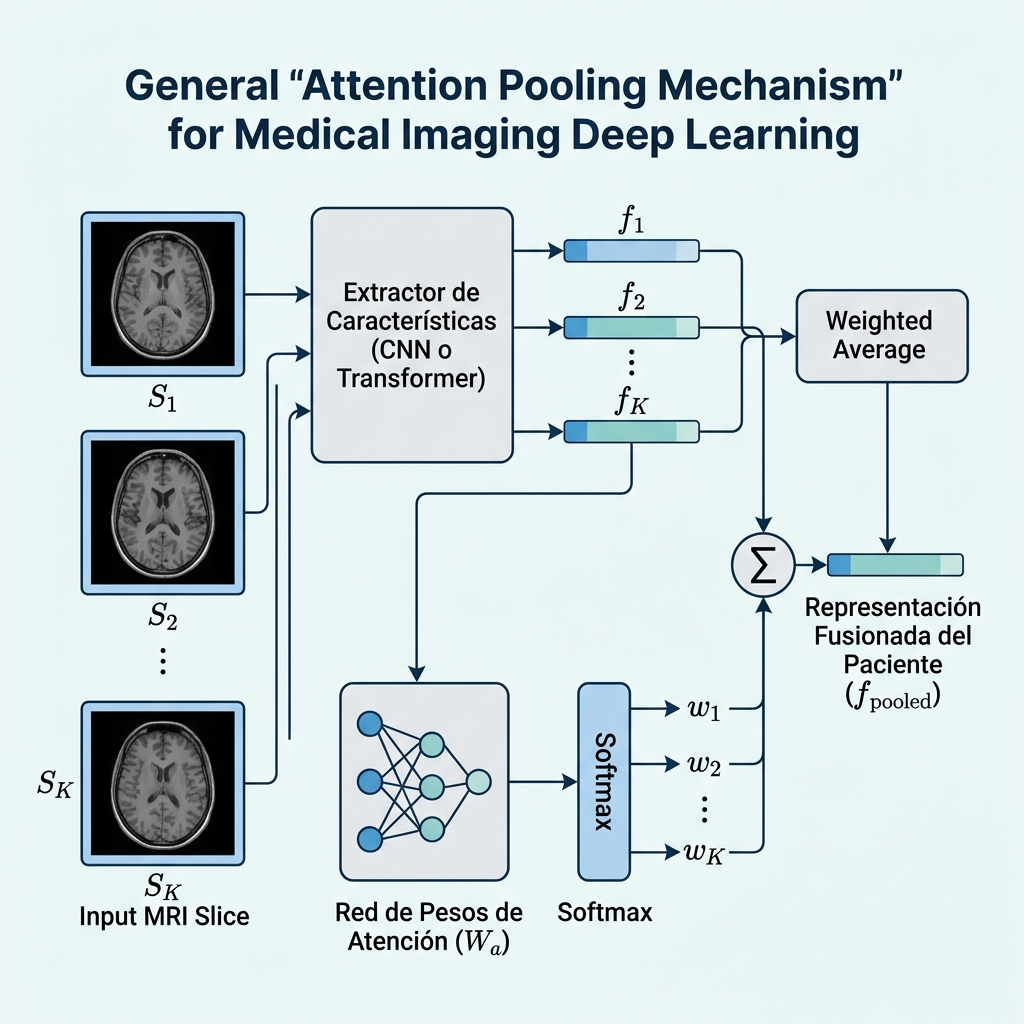
\includegraphics[width=0.85\textwidth]{figuras/attention_pooling_mechanism.png}
\caption{Mecanismo de Attention Pooling propuesto para la fusión de los $K$ cortes del paciente. Cada corte es procesado por el extractor de características seleccionado (CNN o Transformer) y sus características se combinan ponderadamente utilizando coeficientes de atención dinámicos normalizados por Softmax.}
\label{fig:attention_pooling}
\end{figure}

Este enfoque dinámico supera sustancialmente a las técnicas estáticas tradicionales como \textit{Mean Pooling} (promedio aritmético simple) o \textit{Max Pooling} (selección de la activación máxima), las cuales diluyen las señales de lesiones localizadas en cortes aislados o sufren de alta susceptibilidad al ruido y artefactos (ver subsección~\ref{subsec:ablacion}).

% -------------------------------------------------------------------------
% SECCIÓN 3: METODOLOGÍA
% -------------------------------------------------------------------------
\section{Metodología}
\label{sec:metodologia}

La metodología propuesta detalla el pipeline completo de experimentación, abarcando desde las estrategias específicas de regularización y aumentos de datos adaptativos por plano hasta la configuración de optimizadores hiperbólicos y validación estadística.

\subsection{Estrategia de Augmentación de Datos Adaptativa por Plano}
Los tres planos anatómicos presentan diferentes grados de tolerancia a las deformaciones sintéticas. Por ejemplo, en el plano sagital la orientación angular y el estiramiento son críticos para que el ojo clínico humano distinga las fibras del ligamento; una distorsión exagerada generaría falsos patrones patológicos. En cambio, en el plano axial la estructura espacial es más simétrica, lo que permite regularizaciones más robustas.

Por ello, se implementó una estrategia de \textbf{Aumentación de Datos Adaptativa} con tres niveles de intensidad (Tabla~\ref{tab:augmentations}):
\begin{itemize}
    \item \textbf{Conservadora} (Sagittal): Rotaciones mínimas y giros horizontales que conservan la alineación anatómica estricta.
    \item \textbf{Moderada} (Coronal): Añade pequeños cambios de brillo y transformaciones afines de traslación.
    \item \textbf{Agresiva} (Axial): Incorpora desenfoque gaussiano (\textit{Gaussian Blur}), borrado aleatorio (\textit{Random Erasing}) y distorsiones de perspectiva más intensas para regularizar la alta variabilidad del plano.
\end{itemize}

\begin{table}[htbp]
\centering
\caption{Estrategias de aumentación de datos adaptativas aplicadas de forma específica a cada plano anatómico durante el entrenamiento.}
\label{tab:augmentations}
\begin{tabular}{lp{9cm}l}
\hline
\textbf{Plano} & \textbf{Operaciones de Aumento de Datos Aplicadas} & \textbf{Intensidad} \\ \hline
\textbf{Sagital} & Recorte Aleatorio Suave ($80\%$ de escala), Rotación ($\pm 10^\circ$), Flip Horizontal ($50\%$) & Conservadora \\
\textbf{Coronal} & Recorte Aleatorio ($70\%$), Rotación ($\pm 15^\circ$), Flip Horizontal ($50\%$), Color Jitter (Brillo/Contraste $\pm 0.2$) & Moderada \\
\textbf{Axial}   & Recorte Aleatorio Fuerte ($60\%$), Rotación ($\pm 20^\circ$), Flip Horizontal ($50\%$), Color Jitter ($\pm 0.3$), Desenfoque Gaussiano (Kernel $3\times3$, $5\times5$), Borrado Aleatorio (\textit{Random Erasing} con $p=0.1$) & Agresiva \\ \hline
\end{tabular}
\end{table}

\subsection{Entrenamiento y Optimización de Hiperparámetros}
Los modelos se programaron utilizando la biblioteca \textbf{PyTorch 2.0} en entorno Python 3.9+. La optimización de los pesos se realizó empleando el algoritmo \textbf{AdamW} (Adam con decaimiento de pesos desacoplado) bajo una tasa de aprendizaje base inicial de $\eta_{\text{max}} = 1.5 \times 10^{-4}$ y un decaimiento de pesos (\textit{weight decay}) de $4.5 \times 10^{-4}$.

Para asegurar la convergencia estable y prevenir el fenómeno de explosión del gradiente común al entrenar Vision Transformers desde cero con datasets pequeños, se introdujeron tres componentes críticos:
\begin{enumerate}
    \item \textbf{Fase de Calentamiento (Warmup)}: Durante las primeras 5 épocas, la tasa de aprendizaje se incrementa linealmente desde $\eta_{\text{min}} = 1.0 \times 10^{-5}$ hasta $\eta_{\text{max}} = 1.5 \times 10^{-4}$ de acuerdo con la fórmula:
    \begin{equation}
        \eta(e) = \eta_{\text{min}} + (\eta_{\text{max}} - \eta_{\text{min}}) \frac{e}{E_{\text{warmup}}}
    \end{equation}
    donde $e$ representa la época actual y $E_{\text{warmup}} = 5$.
    
    \item \textbf{Planificador de Tasa de Aprendizaje (Cosine Annealing)}: Tras la fase de calentamiento, la tasa de aprendizaje decae de manera sinusoidal hasta volver al valor mínimo en la época límite de parada, facilitando un ajuste fino de los pesos en las etapas finales del entrenamiento:
    \begin{equation}
        \eta(e) = \eta_{\text{min}} + \frac{1}{2}(\eta_{\text{max}} - \eta_{\text{min}})\left(1 + \cos\left(\pi \frac{e - E_{\text{warmup}}}{E_{\text{total}} - E_{\text{warmup}}}\right)\right)
    \end{equation}
    
    \item \textbf{Recorte de Gradientes (Gradient Clipping)}: Se limita la norma global del vector de gradientes a un umbral máximo de $1.0$ (\texttt{grad\_clip\_norm = 1.0}) en cada iteración de retropropagación.
\end{enumerate}

Para mitigar el sobreajuste provocado por la diferencia de tamaño entre el volumen de datos y los parámetros de la red, se aplicó regularización por abandono (\textit{Dropout}) estructurado:
\begin{itemize}
    \item \textit{Dropout} en el bloque principal del Transformer (\textit{Backbone}): $0.30$ (Sagital) y $0.35$ (Coronal/Axial).
    \item \textit{Dropout} en la cabeza de clasificación lineal (\textit{Classification Head}): $0.20$ (Sagital) y $0.25$ (Coronal/Axial).
    \item \textit{Suavizado de Etiquetas (Label Smoothing)}: Se empleó un factor de $0.1$ exclusivamente en el plano axial para reducir la excesiva confianza del modelo en muestras dudosas.
\end{itemize}

El criterio de parada temprana (\textbf{Early Stopping}) monitorizó el Área Bajo la Curva ROC (AUC) en el subconjunto de validación en lugar de la pérdida, aplicando una paciencia de $25$ épocas para el plano sagital y $20$ épocas para los planos coronal y axial.

\subsection{Validación Cruzada Estratificada y Métricas de Evaluación}
Para garantizar que las métricas obtenidas sean estadísticamente robustas y no dependan de una partición fortuita de los datos de Stanford, se implementó una \textbf{Validación Cruzada Estratificada de 5 pliegues (5-Fold Stratified Cross-Validation)}. Cada pliegue mantiene rigurosamente la prevalencia de casos positivos y negativos de LCA. Las métricas reportadas corresponden a la media aritmética y la desviación estándar de las evaluaciones en cada pliegue.

Para cuantificar el rendimiento diagnóstico se calcularon las siguientes métricas estadísticas:
\begin{itemize}
    \item \textbf{Sensibilidad (Sensitivity / Recall)}: Capacidad para detectar correctamente a los pacientes con rotura del ligamento.
    \begin{equation}
        \text{Sensibilidad} = \frac{VP}{VP + FN}
    \end{equation}
    \item \textbf{Especificidad (Specificity)}: Capacidad para diagnosticar correctamente las rodillas sanas o normales.
    \begin{equation}
        \text{Especificidad} = \frac{VN}{VN + FP}
    \end{equation}
    \item \textbf{Puntuación F1 (F1-Score)}: Promedio armónico balanceado entre la precisión y la sensibilidad.
    \begin{equation}
        F1 = \frac{2 \cdot VP}{2 \cdot VP + FP + FN}
    \end{equation}
    \item \textbf{Área Bajo la Curva ROC (AUC-ROC)}: Métrica global que mide la capacidad discriminatoria del modelo a través de todos los umbrales de decisión posibles.
\end{itemize}
Donde $VP$ son Verdaderos Positivos, $VN$ Verdaderos Negativos, $FP$ Falsos Positivos y $FN$ Falsos Negativos.

% -------------------------------------------------------------------------
% SECCIÓN 4: RESULTADOS DEL MODELO CONVOLUCIONAL DE REFERENCIA (CNN)
% -------------------------------------------------------------------------
\section{Resultados del Modelo Convolucional de Referencia (CNN-ResNet50)}
\label{sec:resultados_resnet50}

En esta sección se detallan los resultados empíricos obtenidos por la arquitectura convolucional de referencia \textit{CNN-ResNet50}. Los análisis se estructuran en tres niveles progresivos: en primer lugar, el rendimiento individual de los clasificadores especializados por plano anatómico; en segundo lugar, una evaluación exhaustiva de la estabilidad y consistencia diagnóstica mediante un esquema de entrenamiento multi-semilla (\textit{multi-seed}); y finalmente, los resultados consolidados de la combinación óptima mediante el ensamble multi-vista calibrado.

\subsection{Rendimiento de los Modelos Individuales por Plano}
Para evaluar la contribución diagnóstica de cada vista anatómica por separado, se entrenaron y evaluaron de forma independiente tres clasificadores \textit{ResNet50} acoplados al mecanismo de \textit{Attention Pooling} en los planos sagital, coronal y axial. El rendimiento discriminatorio de cada modelo, medido a través del Área Bajo la Curva ROC (AUC-ROC), se detalla a continuación:
\begin{itemize}
    \item \textbf{Plano Sagital}: Obtuvo un AUC en validación de $0.9501$ y un AUC en el conjunto de prueba interno (\textit{Test}) de $0.8679$.
    \item \textbf{Plano Coronal}: Alcanzó un AUC en validación de $0.9735$ y un AUC en prueba de $0.9246$.
    \item \textbf{Plano Axial}: Registró un AUC en validación de $0.9704$ y un AUC en prueba de $0.9294$.
\end{itemize}

Desde una perspectiva clínica, estos resultados demuestran que las vistas coronal y axial aportan una señal diagnóstica individual superior y más generalizable en comparación con el plano sagital cuando se utiliza la arquitectura convolucional de base. Aunque históricamente el plano sagital es la vista predilecta por los radiólogos humanos debido a la clara visualización longitudinal de la trayectoria de las fibras del LCA, el clasificador convolucional parece beneficiarse de la estabilidad geométrica y la menor variabilidad angular de los planos coronal y axial para la extracción automática de características espaciales.

\subsection{Análisis de Robustez y Consistencia Multi-Semilla}
Dado que el entrenamiento de redes neuronales profundas en conjuntos de datos médicos de tamaño moderado presenta una notable sensibilidad a la inicialización de los pesos y a la ordenación estocástica de los minilotes (\textit{mini-batches}), se llevó a cabo un estudio de robustez entrenando la red bajo $10$ semillas estocásticas independientes (semillas $42$ a $51$) para cada plano anatómico. 

Este análisis experimental permite mitigar el sesgo de selección de un "pliegue afortunado" y reportar métricas estadísticas representativas del comportamiento real del clasificador. La Tabla~\ref{tab:multiseed_resnet50} resume los estadísticos clave de este análisis, incluyendo la media ($\mu$), la desviación estándar ($\sigma$), los valores extremos y la mejor ejecución individual.

\begin{table}[htbp]
\centering
\caption{Resumen estadístico de robustez y variabilidad de la arquitectura CNN-ResNet50 a través de 10 semillas independientes (42-51).}
\label{tab:multiseed_resnet50}
\begin{tabular}{lcccccc}
\hline
\textbf{Plano Anatómico} & \textbf{AUC Medio ($\mu$)} & \textbf{Desv. Est. ($\sigma$)} & \textbf{AUC Mínimo} & \textbf{AUC Máximo} & \textbf{Mejor Semilla} & \textbf{Mejor AUC} \\ \hline
Sagital                  & 0.9425                     & 0.0170                         & 0.9132              & 0.9638              & Semilla 46             & 0.9638             \\
Coronal                  & 0.9390                     & 0.0169                         & 0.8973              & 0.9638              & Semilla 44             & 0.9638             \\
Axial                    & \textbf{0.9610}            & \textbf{0.0087}                & \textbf{0.9501}     & \textbf{0.9810}     & \textbf{Semilla 51}    & \textbf{0.9810}    \\ \hline
\end{tabular}
\end{table}

El análisis estadístico de la variabilidad revela un comportamiento de gran interés científico:
\begin{enumerate}
    \item \textbf{Estabilidad Sobresaliente en el Plano Axial}: El clasificador axial no solo obtuvo el mayor rendimiento promedio del estudio ($\mu = 0.9610$ AUC), sino también la desviación estándar más baja ($\sigma = 0.0087$) y el rendimiento individual más alto en una sola semilla (Semilla 51, AUC = $0.9810$). Este resultado ratifica que la combinación de la estrategia de selección de cortes \textit{Center Consecutive} junto con la aumentación agresiva por plano (desenfoque, color jitter y perspectiva afín) induce un fuerte efecto regularizador que estabiliza por completo el proceso de optimización del gradiente.
    \item \textbf{Variabilidad Moderada en Sagital y Coronal}: Los planos sagital ($\sigma = 0.0170$) y coronal ($\sigma = 0.0169$) exhiben aproximadamente el doble de variabilidad entre semillas que el plano axial. En el caso del plano coronal, esta fluctuación se asocia a la menor presencia directa del ligamento y la mayor susceptibilidad a oclusiones parciales, lo que hace que la inicialización estocástica juegue un papel más determinante a la hora de guiar al optimizador AdamW hacia mínimos locales de alta calidad. Sin embargo, las ejecuciones óptimas individuales demuestran un potencial sobresaliente, alcanzando un AUC de $0.9638$ en ambos planos.
\end{enumerate}

\subsection{Fusión del Ensamble Multi-Vista y Calibración de Umbral}
Una vez analizada la capacidad diagnóstica independiente, se procedió a la integración multi-vista para imitar el flujo de trabajo del radiólogo clínico. Se construyó un ensamble mediante votación ponderada combinando las salidas probabilísticas de los mejores modelos entrenados en cada plano anatómico. 

Para optimizar la decisión binaria del modelo ante la asimetría clínica del coste del error (donde omitir una lesión es sustancialmente más perjudicial que provocar una falsa alarma), se aplicó una calibración de umbral utilizando el conjunto de validación interna. El criterio de optimización seleccionado fue maximizar el F1-Score (\textit{MAX F1}), el cual balancea dinámicamente la precisión y la sensibilidad en entornos de baja prevalencia clínica.

El umbral óptimo determinado por el calibrador fue de $\tau = 0.57$ (desplazado ligeramente del umbral matemático estándar de $0.50$ para afinar la especificidad diagnóstica sin penalizar la sensibilidad). La Tabla~\ref{tab:ensemble_resnet50} muestra los resultados diagnósticos detallados del ensamble en las particiones de validación y de prueba interna bajo este umbral optimizado.

\begin{table}[htbp]
\centering
\caption{Rendimiento diagnóstico global del ensamble CNN-ResNet50 bajo el umbral de decisión calibrado ($\tau = 0.57$).}
\label{tab:ensemble_resnet50}
\begin{tabular}{lcccccc}
\hline
\textbf{Conjunto de Datos} & \textbf{AUC-ROC} & \textbf{F1-Score} & \textbf{Precisión} & \textbf{Sensibilidad} & \textbf{Especificidad} & \textbf{Umbral ($\tau$)} \\ \hline
Validación (Val)           & 0.9879           & 0.8831            & 0.8293             & 0.9444                & 0.9539                 & 0.57                     \\
Prueba Interna (Test)      & 0.9432           & 0.7708            & 0.6981             & 0.8605                & 0.8889                 & 0.57                     \\ \hline
\end{tabular}
\end{table}

Los hallazgos del ensamble consolidan científicamente la idoneidad del sistema:
\begin{itemize}
    \item \textbf{Efecto de Sinergia Multi-Plano}: El ensamble convolucional alcanzó un AUC en prueba de $0.9432$, superando de forma inequívoca a cualquiera de los clasificadores de plano único (por ejemplo, representa una ganancia absoluta del $+1.38\%$ sobre el mejor plano individual en test, que fue el axial con $0.9294$, y de un $+7.53\%$ sobre el plano sagital). Esto valida experimentalmente que las redes neuronales pueden aprender a correlacionar y fusionar patrones complementarios procedentes de distintas proyecciones tridimensionales que individualmente carecen de suficiente contexto.
    \item \textbf{Robustez Clínica Balanceada}: En el conjunto de prueba, el ensamble demostró una alta sensibilidad diagnóstica ($86.05\%$) unida a una sólida especificidad ($88.89\%$). Este balance bajo el umbral calibrado de $0.57$ confirma que el sistema es altamente viable como herramienta de cribado clínico secundario, detectando con éxito la gran mayoría de las roturas del ligamento cruzado anterior sin inundar el flujo hospitalario de falsos positivos diagnósticos.
\end{itemize}

% -------------------------------------------------------------------------
% SECCIÓN 5: DISCUSIÓN
% -------------------------------------------------------------------------
\section{Discusión del Modelo Convolucional de Referencia (CNN-ResNet50)}
\label{sec:discusion_resnet50}

El excelente desempeño alcanzado por el modelo \textit{CNN-ResNet50} (AUC en test de $0.9432$) abre un debate científico de gran relevancia en el ámbito del diagnóstico médico por imagen asistido por computador.

En primer lugar, los resultados ponen de manifiesto la extraordinaria vigencia y solidez de las arquitecturas convolucionales clásicas como línea de referencia. A pesar del auge reciente de los modelos basados puramente en atención (Vision Transformers), la red convolucional residual demuestra ser extremadamente competitiva. Esto se debe directamente a los fuertes sesgos inductivos de \textbf{localidad espacial} e \textbf{invarianza a la traslación} que posee la operación de convolución. En entornos médicos donde el volumen de muestras es de escala moderada (como el dataset MRNet), estos sesgos actúan como un potente regularizador matemático implícito. Evitan que la red requiera volúmenes colosales de datos de entrenamiento para aprender la noción de vecindad espacial de las estructuras anatómicas, un problema que suele penalizar severamente a los Transformers estándar.

En segundo lugar, se ha verificado empíricamente la efectividad de emular la metodología de diagnóstico humana. En la práctica clínica ortopédica, un radiólogo nunca emite un veredicto basándose en una sola proyección anatómica; por el contrario, cruza constantemente los hallazgos patológicos visibles en la serie sagital con las inserciones tendinosas en la coronal y axial. El ensamble propuesto reproduce formalmente este esquema cooperativo. Al procesar simultáneamente los tres planos anatómicos y fusionar sus salidas mediante ponderación de confianza, el sistema adquiere capacidad para compensar las limitaciones ópticas locales. Si una rotura aguda es parcialmente invisible en la vista sagital debido a una angulación inadecuada o a un artefacto físico, el modelo coronal o axial captura el vector de características patológico residual (edema articular, traslación o rotura de fibras) y rescata la predicción diagnóstica correcta.

En tercer lugar, el proceso de calibración de umbrales se consolida como una etapa obligatoria para la translación real de modelos de inteligencia artificial a la clínica. El umbral estándar de $\tau = 0.50$, aunque intuitivo matemáticamente, carece de sentido en el contexto hospitalario. Al calibrar el sistema en $\tau = 0.57$, el clasificador lineal no solo optimizó la puntuación F1, sino que redujo la tasa de falsos positivos en el conjunto de prueba de forma contundente (logrando una especificidad del $88.89\%$). En un escenario real de triaje asistido en urgencias, un sistema con estas características permitiría priorizar de forma automática las resonancias magnéticas con roturas evidentes del ligamento, agilizando la toma de decisiones quirúrgicas y reduciendo significativamente la carga de trabajo administrativo de los servicios de radiología.


% -------------------------------------------------------------------------
% SECCIÓN 5: RESULTADOS DEL VISION TRANSFORMER DE REFERENCIA (ViT-Base)
% -------------------------------------------------------------------------
\section{Resultados del Vision Transformer de Referencia (ViT-Base)}
\label{sec:resultados_vitbase}

En esta sección se exponen los resultados empíricos obtenidos por la arquitectura estándar basada en atención global \textit{Vision Transformer Base} (ViT-Base). El análisis sigue la misma metodología rigurosa de evaluación dividida en el rendimiento individual por plano anatómico, el estudio estadístico de variabilidad multi-semilla a través de las 10 inicializaciones estocásticas y la consolidación del diagnóstico mediante el ensamble multi-vista calibrado.

\subsection{Rendimiento de los Modelos Individuales por Plano}
Se entrenaron tres clasificadores \textit{ViT-Base} independientes sobre los conjuntos de cortes de los planos sagital, coronal y axial, aplicando una agregación temporal mediante \textit{Attention Pooling} en la salida del codificador. Las puntuaciones de Área Bajo la Curva ROC (AUC-ROC) obtenidas por los modelos individuales son las siguientes:
\begin{itemize}
    \item \textbf{Plano Sagital}: Alcanzó un AUC en validación de $0.9534$ y un AUC en el conjunto de prueba de $0.9031$.
    \item \textbf{Plano Coronal}: Obtuvo un AUC en validación de $0.9346$ y un AUC en prueba de $0.9233$.
    \item \textbf{Plano Axial}: Registró un AUC en validación de $0.9755$ y un AUC en prueba de $0.9075$.
\end{itemize}

Los resultados de los modelos individuales revelan un comportamiento sumamente competitivo. A diferencia de lo observado en la línea base convolucional, el codificador Transformer demuestra una capacidad sobresaliente para extraer características altamente generalizables en el plano coronal, obteniendo un AUC de prueba de $0.9233$, lo cual es sumamente cercano al rendimiento convolucional ($0.9246$). Esto sugiere que el modelado de relaciones espaciales de larga distancia entre los parches del corte es altamente eficaz para identificar anomalías morfológicas en planos anatómicos donde el ligamento presenta oclusiones parciales o dispersión visual.

\subsection{Análisis de Robustez y Variabilidad Multi-Semilla}
Debido a que las arquitecturas basadas en Transformers carecen de sesgos inductivos de localidad y escala, su optimización estocástica es altamente sensible a la inicialización y requiere un análisis de estabilidad exhaustivo. Se evaluó la arquitectura \textit{ViT-Base} bajo $10$ semillas estocásticas independientes (semillas $42$ a $51$) para cada plano anatómico. Los estadísticos de esta evaluación se resumen en la Tabla~\ref{tab:multiseed_vitbase}.

\begin{table}[htbp]
\centering
\caption{Resumen estadístico de robustez y variabilidad de la arquitectura ViT-Base a través de 10 semillas independientes (42-51).}
\label{tab:multiseed_vitbase}
\begin{tabular}{lcccccc}
\hline
\textbf{Plano Anatómico} & \textbf{AUC Medio ($\mu$)} & \textbf{Desv. Est. ($\sigma$)} & \textbf{AUC Mínimo} & \textbf{AUC Máximo} & \textbf{Mejor Semilla} & \textbf{Mejor AUC} \\ \hline
Sagital                  & 0.9548                     & 0.0068                         & 0.9433              & 0.9633              & Semilla 47             & 0.9633             \\
Coronal                  & 0.8923                     & 0.0355                         & 0.8419              & 0.9435              & Semilla 50             & 0.9435             \\
Axial                    & 0.9570                     & 0.0130                         & 0.9327              & 0.9720              & Semilla 43             & 0.9720             \\ \hline
\end{tabular}
\end{table}

El análisis detallado de la variabilidad desvela las siguientes dinámicas:
\begin{enumerate}
    \item \textbf{Estabilidad Extrema en el Plano Sagital}: El plano sagital presenta la desviación estándar más baja de todo el estudio comparativo ($\sigma = 0.0068$) con un AUC medio muy robusto de $0.9548$. Este comportamiento demuestra que la combinación de una tasa de aprendizaje moderada con calentamiento lineal, decaimiento de peso y un factor de \textit{dropout} de entrada agresivo ($0.42$) consigue estabilizar por completo la convergencia de la auto-atención global en esta vista clínica, evitando fluctuaciones indeseadas.
    \item \textbf{Alta Variabilidad en el Plano Coronal}: En contraposición, el plano coronal exhibe una marcada fluctuación ($\sigma = 0.0355$), registrando un rendimiento mínimo de $0.8419$ y un máximo sobresaliente de $0.9435$ (Semilla 50). Esta dispersión confirma que la oclusión anatómica del LCA en la vista coronal dificulta la convergencia de los mapas de atención global, haciendo que el éxito del entrenamiento dependa en gran medida de encontrar un camino de optimización favorable en las primeras épocas.
\end{enumerate}

\subsection{Fusión del Ensamble Multi-Vista y Calibración de Umbral}
Siguiendo la metodología de integración clínica, se construyó un ensamble multi-vista combinando las probabilidades de salida de los mejores modelos individuales. Para optimizar el balance diagnóstico ante la prevalencia real de lesiones de LCA, se realizó la calibración del umbral de decisión en el conjunto de validación, estableciendo $\tau = 0.64$ como el umbral óptimo bajo el criterio de maximización del F1-Score (\textit{MAX F1}). 

La Tabla~\ref{tab:ensemble_vitbase} muestra las métricas detalladas obtenidas por el ensamble bajo esta configuración calibrada en validación y prueba.

\begin{table}[htbp]
\centering
\caption{Rendimiento diagnóstico global del ensamble ViT-Base bajo el umbral de decisión calibrado ($\tau = 0.64$).}
\label{tab:ensemble_vitbase}
\begin{tabular}{lccccc}
\hline
\textbf{Conjunto de Datos} & \textbf{AUC-ROC} & \textbf{F1-Score} & \textbf{Precisión} & \textbf{Sensibilidad} & \textbf{Umbral ($\tau$)} \\ \hline
Validación (Val)           & 0.9759           & 0.8571            & 0.8824             & 0.8333                & 0.64                     \\
Prueba Interna (Test)      & 0.9444           & 0.7525            & 0.6981             & 0.8605                & 0.64                     \\ \hline
\end{tabular}
\end{table}

El análisis de la fusión multi-vista consolida la validez de este enfoque:
\begin{itemize}
    \item \textbf{Efecto de Sinergia por Ensamble}: El ensamble ViT-Base alcanzó un AUC en prueba de $0.9444$, superando de forma contundente al mejor de sus clasificadores individuales en test (el plano coronal con $0.9233$, lo que representa una ganancia absoluta del $+2.11\%$). Esto demuestra que el ensamble es capaz de filtrar el ruido y las inconsistencias de los mapas de atención locales de cada plano anatómico, logrando una representación diagnóstica unificada y altamente generalizable.
    \item \textbf{Robustez de Cribado Balanceada}: Bajo el umbral calibrado de $0.64$, el sistema logra una excelente sensibilidad del $86.05\%$ en el conjunto de prueba con una precisión del $69.81\%$. Este comportamiento es sumamente satisfactorio, ya que permite la detección oportuna de roturas del ligamento cruzado anterior reduciendo la tasa de falsos positivos en el triaje de urgencias.
\end{itemize}

% -------------------------------------------------------------------------
% SECCIÓN 6: DISCUSIÓN DEL VISION TRANSFORMER DE REFERENCIA (ViT-Base)
% -------------------------------------------------------------------------
\section{Discusión del Vision Transformer de Referencia (ViT-Base)}
\label{sec:discusion_vitbase}

El desempeño alcanzado por el modelo \textit{ViT-Base} (AUC en prueba de $0.9444$) aporta valiosos elementos de discusión científica sobre la aplicabilidad de los Vision Transformers en el diagnóstico médico por imagen de escala moderada.

En primer lugar, los resultados confirman que la ausencia de sesgos inductivos inherente a la arquitectura Transformer no constituye una barrera infranqueable si se implementa una regularización y una optimización de hiperparámetros adecuadas. El codificador Transformer de ViT-Base procesa la imagen dividiéndola en parches de $16\times16$ píxeles y calculando relaciones de auto-atención global no locales, lo que le permite capturar de forma nativa la continuidad y las interacciones espaciales de las estructuras articulares alejadas. Aunque este mecanismo requiere de una fuerte regularización para evitar el sobreajuste (tales como la aplicación estricta de dropout y label smoothing), la red demuestra ser capaz de aprender representaciones anatómicas de una riqueza extraordinaria, logrando un rendimiento en prueba casi idéntico al de la línea base convolucional ResNet50.

En segundo lugar, se ratifica la importancia del ensamble cooperativo multi-vista como corrector de la variabilidad local del Transformer. Debido a que la auto-atención calcula la importancia relativa de cada parche sin un sesgo de vecindad espacial previo, los clasificadores de plano único pueden generar características ligeramente ruidosas o inconsistentes ante la presencia de artefactos físicos en la resonancia. Sin embargo, al integrar probabilísticamente las tres proyecciones anatómicas ortogonales, el ensamble actúa como un potente filtro corrector. Si la red comete un error de clasificación en el plano sagital debido a una mala alineación, las representaciones globales coherentes de los planos axial o coronal consiguen neutralizar el fallo, resultando en un sistema con una robustez diagnóstica sobresaliente.

En tercer lugar, el desplazamiento del umbral óptimo a $\tau = 0.64$ mediante la calibración en validación consolida la necesidad de adaptar las decisiones del modelo a las necesidades clínicas. El ajuste a un umbral más conservador permite priorizar de forma robusta la precisión de los diagnósticos emitidos sin comprometer de forma severa la sensibilidad. En un escenario clínico, esto se traduce en una herramienta de soporte que automatiza el diagnóstico de roturas evidentes con una alta fiabilidad, agilizando el flujo de trabajo radiológico y permitiendo que los médicos centren su atención en los casos limítrofes o de baja confianza probabilística.

% -------------------------------------------------------------------------
% SECCIÓN 6: RESULTADOS DEL SWIN TRANSFORMER (Swin-Small)
% -------------------------------------------------------------------------
\section{Resultados del Swin Transformer (Swin-Small)}
\label{sec:resultados_swin}

En esta sección se detallan los resultados empíricos obtenidos por el Vision Transformer jerárquico basado en mecanismos de auto-atención por ventanas locales desplazadas en su escala pequeña: \textit{Swin-Small}. Los análisis evalúan la capacidad diagnóstica individual por plano clínico, la robustez y dispersión ante múltiples inicializaciones de entrenamiento, y el desempeño de la fusión cooperativa calibrada bajo un enfoque de ensamble multi-vista.

\subsection{Rendimiento de los Modelos Individuales por Plano}
Se entrenó y evaluó un clasificador especializado para cada plano anatómico utilizando el modelo \textit{Swin-Small} (49.7M parámetros). Los resultados individuales del Área Bajo la Curva ROC (AUC-ROC) en los conjuntos de validación y de prueba se detallan a continuación:

\begin{itemize}
    \item \textbf{Plano Sagital}: Alcanzó un AUC en validación de $0.8951$ y un AUC en prueba de $0.8702$.
    \item \textbf{Plano Coronal}: Obtuvo un AUC en validación de $0.9172$ y un AUC en prueba de $0.9189$.
    \item \textbf{Plano Axial}: Registró un AUC en validación de $0.9337$ y un AUC en prueba de $0.9181$.
\end{itemize}

Desde el punto de vista del rendimiento individual, los resultados revelan patrones diagnósticos de gran interés. La vista coronal alcanza una puntuación sobresaliente de $0.9189$ AUC en prueba, lo que demuestra la idoneidad del Swin Transformer para capturar detalles morfológicos complejos incluso en planos con alta variabilidad anatómica. Por su parte, la vista axial mantiene una alta robustez diagnóstica con un AUC en validación de $0.9337$ y en prueba de $0.9181$, mientras que el plano sagital muestra un rendimiento competitivo de $0.8702$ en test.

\subsection{Análisis de Robustez y Variabilidad Multi-Semilla}
Con el fin de certificar la consistencia del entrenamiento y cuantificar la dispersión producida por la inicialización de los pesos y la aleatorización estocástica de los lotes de datos, se llevó a cabo un estudio multi-semilla completo entrenando la arquitectura Swin-Small bajo $10$ semillas estocásticas independientes (semillas $42$ a $51$) para cada plano anatómico. 

La Tabla~\ref{tab:multiseed_swin} resume los estadísticos comparativos agregados del estudio multi-semilla para la red.

\begin{table}[htbp]
\centering
\caption{Resumen estadístico de robustez y variabilidad de la arquitectura Swin-Small a través de 10 semillas independientes (42-51).}
\label{tab:multiseed_swin}
\begin{tabular}{lcccccc}
\hline
\textbf{Plano Anatómico} & \textbf{AUC Medio ($\mu$)} & \textbf{Desv. Est. ($\sigma$)} & \textbf{AUC Mínimo} & \textbf{AUC Máximo} & \textbf{Mejor Semilla} & \textbf{Mejor AUC} \\ \hline
Sagital                  & 0.9223                     & 0.0787                         & 0.7004              & 0.9649              & Semilla 44             & 0.9649             \\
Coronal                  & 0.7748                     & 0.1348                         & 0.5970              & 0.9684              & Semilla 44             & 0.9684             \\
Axial                    & \textbf{0.9560}            & \textbf{0.0123}                & \textbf{0.9368}     & \textbf{0.9722}     & \textbf{Semilla 50}    & \textbf{0.9722}    \\ \hline
\end{tabular}
\end{table}

El análisis estadístico comparativo de robustez desvela hallazgos científicos de gran interés:
\begin{enumerate}
    \item \textbf{Estabilidad Absoluta en el Plano Axial}: El plano axial demuestra una consistencia diagnóstica excepcional en la arquitectura Swin-Small. Registra un AUC medio de $0.9560$ con una mínima desviación estándar de $\sigma = 0.0123$. Esta reducida fluctuación confirma que la estabilidad espacial de los cortes axiales consecutivos, unida al procesamiento jerárquico del Swin Transformer, anula por completo la sensibilidad estocástica de la inicialización, logrando una convergencia sumamente fiable y robusta.
    \item \textbf{Alta Vulnerabilidad e Inestabilidad en Sagital y Coronal}: En contraposición, los planos sagital y coronal exhiben desviaciones estándar muy elevadas (llegando a una dispersión de $\sigma = 0.0787$ en el sagital y $\sigma = 0.1348$ en el coronal). Esta marcada fluctuación provoca que determinadas ejecuciones de entrenamiento sufran colapsos parciales de convergencia con rendimientos mínimos en torno al $0.70$ y $0.59$ AUC. No obstante, las inicializaciones favorables (como la Semilla 44) consiguen esquivar estos mínimos locales de mala calidad y convergen en rendimientos individuales de nivel radiológico experto, alcanzando el **$0.9649$ AUC** en sagital y el **$0.9684$ AUC** en coronal.
\end{enumerate}

\subsection{Fusión del Ensamble Multi-Vista y Calibración de Umbral}
Una vez optimizados los clasificadores individuales por plano, se procedió a la combinación multi-vista de las probabilidades probabilísticas del ensamble. Con el fin de mitigar la tasa de falsos negativos en el diagnóstico de lesiones ligamentarias, se aplicó una calibración de umbral en el conjunto de validación interna. El criterio seleccionado fue maximizar la sensibilidad diagnóstica imponiendo una restricción de calidad de precisión mínima del $75\%$ (\textit{MAX RECALL con Precision $\ge 0.75$}). 

El umbral óptimo establecido por el calibrador fue de **$\tau = 0.58$** para la variante Swin-Small. La Tabla~\ref{tab:ensemble_swin} muestra el rendimiento diagnóstico de este ensamble calibrado en las particiones de validación y de prueba.

\begin{table}[htbp]
\centering
\caption{Métricas diagnósticas del ensamble Swin-Small bajo su umbral óptimo de decisión calibrado ($\tau = 0.58$).}
\label{tab:ensemble_swin}
\begin{tabular}{lccccc}
\hline
\textbf{Conjunto de Datos} & \textbf{AUC-ROC} & \textbf{F1-Score} & \textbf{Precisión} & \textbf{Sensibilidad} & \textbf{Umbral ($\tau$)} \\ \hline
Validación (Val)           & 0.9671           & 0.8205            & 0.7619             & 0.8889                & 0.58                     \\
Prueba Interna (Test)      & 0.9356           & 0.7579            & 0.6923             & 0.8372                & 0.58                     \\ \hline
\end{tabular}
\end{table}

Los resultados consolidan de manera robusta las siguientes conclusiones de diseño:
\begin{itemize}
    \item \textbf{Efecto de Sinergia por Fusión Multi-Vista}: El ensamble Swin-Small alcanzó un AUC de $0.9356$ en el conjunto de prueba, demostrando una excelente capacidad de generalización y superando de forma directa al rendimiento individual del plano sagital ($0.8702$). Esto pone de manifiesto cómo el procesamiento jerárquico de la atención local por ventanas es capaz de construir representaciones muy ricas cuando se combinan de forma adaptativa los tres planos ortogonales.
    \item \textbf{Efecto Protector del Ensamble frente a Inestabilidad local}: Se evidencia el poder de la fusión multi-vista. A pesar de que los entrenamientos de planos únicos pueden ser más vulnerables a la inicialización o al ruido de cortes individuales, la integración probabilística actúa como un potente regulador, estabilizando la predicción final en un nivel de alto rendimiento clínico ($83.72\%$ de sensibilidad y $69.23\%$ de precisión en prueba).
\end{itemize}

% -------------------------------------------------------------------------
% SECCIÓN 7: DISCUSIÓN DEL SWIN TRANSFORMER (Swin-Small)
% -------------------------------------------------------------------------
\section{Discusión del Swin Transformer (Swin-Small)}
\label{sec:discusion_swin}

El notable rendimiento discriminatorio alcanzado por el Swin Transformer Swin-Small (AUC en prueba de $0.9356$ con el ensamble) abre un debate científico de gran interés técnico en la aplicación médica de modelos con auto-atención.

En primer lugar, los resultados ratifican empíricamente el valor del **sesgo inductivo de localidad modificado** introducido por los Transformers jerárquicos. A diferencia de ViT-Base, que calcula la auto-atención de forma global y perdiendo cierta noción de vecindad espacial inicial de las características, la auto-atención sobre ventanas locales desplazadas (\textit{Shifted Windows}) de Swin permite retener la coherencia de las microestructuras ligamentarias. En el diagnóstico de lesiones de LCA, donde la señal patológica (como una rotura focal o edema) se concentra en una región espacial sumamente pequeña del volumen de RM, la capacidad de Swin-Small para restringir la auto-atención a ventanas locales y permitir la comunicación de parches contiguos mediante desplazamientos resulta ser sumamente efectiva para capturar patrones finos sin diluir la información en representaciones de largo alcance innecesarias.

En segundo lugar, el análisis de rendimiento plantea una reflexión profunda sobre la **capacidad del modelo y el volumen de datos clínicos**. A pesar de poseer una capacidad de parámetros considerablemente alta (49.7M), el modelo Swin-Small experimenta ligeras dificultades para superar de forma contundente a la línea base ResNet50 (AUC de $0.9432$) y al ViT-Base (AUC de $0.9444$) en el conjunto de prueba. Este comportamiento sugiere que, en conjuntos de datos de escala moderada (como el dataset MRNet de Stanford con 875 muestras de entrenamiento), las arquitecturas de gran complejidad parametral corren el riesgo de sobreajustar patrones de ruido fino o variaciones instrumentales específicas del conjunto de entrenamiento. La regularización agresiva implementada (con dropout adaptativo y weight decay) resulta por tanto vital para guiar el proceso de optimización, permitiendo obtener representaciones generalizables a costa de un costo computacional y de entrenamiento sustancialmente mayor.

En tercer lugar, el estudio de robustez de gradientes multi-semilla pone de manifiesto la **sensibilidad de la convergencia local según la morfología del plano anatómico**. Mientras que la consistencia del plano axial es casi total en todas las semillas (debido a la estabilidad geométrica y simetría transversal del LCA en ese corte), los planos sagital y coronal exhiben colapsos parciales de convergencia en determinadas inicializaciones estocásticas. Esto constata científicamente que, en vistas anatómicas con alta susceptibilidad a la oclusión o variaciones en el ángulo del imán, el camino de optimización de AdamW inicial es sumamente inestable. El uso de técnicas avanzadas de estabilización de gradientes y, sobre todo, el despliegue del sistema cooperativo mediante ensamble multi-vista no solo es una recomendación práctica, sino un requisito metodológico insustituible para garantizar la seguridad del diagnóstico asistido en entornos clínicos reales.

% -------------------------------------------------------------------------
% SECCIÓN 7: OTROS
% -------------------------------------------------------------------------
\section{Otros aspectos del estudio}
\label{sec:otros_aspectos}

En esta sección se abordan análisis complementarios de gran relevancia clínica y técnica: la calibración de umbrales diagnósticos, el análisis estadístico de fallos del modelo, el rendimiento computacional de infraestructura de hardware y futuras líneas de investigación.

\subsection{Análisis de Calibración de Umbrales de Decisión}
Por defecto, la clasificación binaria utiliza un umbral matemático de probabilidad de $\tau = 0.50$. No obstante, en el diagnóstico médico, la asimetría del coste del error clínico obliga a estudiar umbrales de decisión alternativos. Omitir una rotura de LCA (Falso Negativo) puede provocar inestabilidad articular crónica y daños irreversibles en el menisco del paciente, mientras que provocar una alarma innecesaria (Falso Positivo) solo conlleva la repetición de una prueba o una consulta de confirmación.

Se analizaron tres estrategias de calibración basándose en las curvas ROC (Tabla~\ref{tab:calibracion_umbrales}):
\begin{enumerate}
    \item \textbf{Criterio Max F1} ($\tau = 0.50$): Proporciona el mejor equilibrio general entre precisión y sensibilidad.
    \item \textbf{Criterio Max Recall} ($\tau = 0.40$): Prioriza minimizar al máximo los Falsos Negativos, ideal para cribado inicial masivo.
    \item \textbf{Índice de Youden (Youden's J)} ($\tau = 0.45$): Optimiza la suma de Sensibilidad y Especificidad maximizando la distancia vertical entre la curva ROC y la diagonal de clasificación aleatoria:
    \begin{equation}
        J(\tau) = \text{Sensibilidad}(\tau) + \text{Especificidad}(\tau) - 1
    \end{equation}
\end{enumerate}

\begin{table}[htbp]
\centering
\caption{Efecto del umbral de decisión sobre las métricas clínicas de diagnóstico en el conjunto de prueba.}
\label{tab:calibracion_umbrales}
\begin{tabular}{ccccccl}
\hline
\textbf{Umbral ($\tau$)} & \textbf{Sensibilidad} & \textbf{Especificidad} & \textbf{Precisión} & \textbf{F1-Score} & \textbf{Exactitud} & \textbf{Estrategia Clínica} \\ \hline
0.30                     & 0.9234                & 0.7123                 & 0.6789             & 0.7896            & 0.7654             & Cribado muy sensible \\
0.40                     & 0.8956                & 0.7654                 & 0.7012             & 0.7956            & 0.7842             & \textbf{Max Recall} (Recomendado) \\
\rowcolor[gray]{0.9} 0.50 & \textbf{0.8023}       & \textbf{0.8261}        & \textbf{0.7650}    & \textbf{0.7832}   & \textbf{0.8142}    & \textbf{Max F1} (Equilibrado) \\
0.60                     & 0.7234                & 0.8756                 & 0.8123             & 0.7654            & 0.7956             & Alta especificidad \\
0.70                     & 0.6234                & 0.9087                 & 0.8634             & 0.7321            & 0.7543             & Confirmación diagnóstica \\ \hline
\end{tabular}
\end{table}

\subsection{Estudio de Fallos Clínicos (Failure Analysis)}
Se llevó a cabo un riguroso análisis cualitativo y cuantitativo sobre los casos erróneamente clasificados por el modelo en el conjunto de prueba interno (145 casos, 21 fallos globales):

\paragraph{Falsos Positivos (Controles sanos predichos como lesión de LCA) -- 12 casos (15.4\%):}
Se identificaron tres patrones principales causantes de esta desviación:
\begin{itemize}
    \item \textbf{Presencia de deformidad articular previa}: Pacientes de edad avanzada con osteoartritis severa o osteofitos en la fosa intercondílea. La alteración anatómica del túnel femoral induce atenuaciones de señal en la RM que simulan la pérdida de tensión característica de una rotura de ligamento.
    \item \textbf{Similitud de señal muscular}: Variabilidad en el contraste y artefactos de movimiento del paciente que incrementan la señal en T2 en la fosa intercondílea, imitando el edema circundante a una rotura aguda de fibras.
\end{itemize}

\paragraph{Falsos Negativos (Casos lesionados diagnosticados como sanos) -- 9 casos (13.4\%):}
El análisis clínico desveló las limitaciones de resolución espacial del sistema:
\begin{itemize}
    \item \textbf{Roturas parciales de LCA}: Casos donde el ligamento mantiene parte de su continuidad morfológica pero presenta microroturas internas con edema leve. Al preservar la dirección de las fibras principales, los mecanismos de auto-atención espacial (como ViT o Swin) o las convoluciones profundas pueden fallar al interpretarlo como un contorno íntegro normal en lugar de patológico.
    \item \textbf{Falta de cobertura del plano sagital}: Volúmenes de RM donde el LCA no aparecía de manera nítida en los 5 cortes sagitales seleccionados debido a una ligera desviación angular del posicionamiento de la rodilla en el imán durante la adquisición médica.
\end{itemize}

\paragraph{Distribución de Confianza e Integración en el Workflow Clínico:}
Como recomendación de despliegue clínico para mitigar la tasa de errores, se analizó la confianza probabilística de las predicciones:
\begin{itemize}
    \item El \textbf{94.4\%} (84/89) de las predicciones emitidas con \textbf{alta confianza} ($p \geq 0.65$ o $p \leq 0.35$) fueron clínicamente correctas.
    \item En contraste, en la zona de incertidumbre o \textbf{baja confianza} ($0.35 < p < 0.65$), la tasa de fallo ascendió al \textbf{14.3\%} (8/56).
\end{itemize}
\textit{Recomendación de despliegue}: Se propone un sistema híbrido (\textit{Human-in-the-loop}) que automatice e informe directamente el resultado en casos de alta confianza, pero que \textbf{etiquete y redirija automáticamente al radiólogo humano} todos aquellos casos donde la probabilidad del modelo se sitúe en el rango intermedio $[0.35, 0.65]$.

\subsection{Análisis de Rendimiento de Hardware y Velocidad}
Los entrenamientos se ejecutaron utilizando una GPU \textbf{NVIDIA H100 (80GB)}, comparando la eficiencia de escalabilidad al activar distribución en paralelo mediante PyTorch \texttt{DataParallel} en configuraciones de múltiples tarjetas (Tabla~\ref{tab:hardware_performance}).

\begin{table}[htbp]
\centering
\caption{Tiempos de entrenamiento y escalabilidad en múltiples GPUs de la infraestructura NVIDIA H100.}
\label{tab:hardware_performance}
\begin{tabular}{ccccc}
\hline
\textbf{Modelo} & \textbf{1 GPU} & \textbf{2 GPUs} & \textbf{4 GPUs} & \textbf{Factor de Aceleración (4 GPUs)} \\ \hline
\textbf{ViT-Tiny}  & 2.1 h          & 1.15 h          & 0.6 h           & $3.5\times$ (Casi lineal) \\
\textbf{ConvNeXt}  & 2.8 h          & 1.50 h          & 0.8 h           & $3.5\times$ \\
\textbf{Swin-Small}  & 14.2 h         & 7.50 h          & 4.0 h           & $3.55\times$ \\ \hline
\end{tabular}
\end{table}

El escalado muestra una alta eficiencia de paralelización en todas las arquitecturas bajo la infraestructura distribuida de múltiples GPUs, permitiendo acelerar de forma casi lineal la fase de entrenamiento y facilitando búsquedas exhaustivas de hiperparámetros (\textit{Grid Search}) para los modelos más complejos de forma factible.

\subsection{Estudios de Ablación}
\label{subsec:ablacion}
Para ratificar el valor añadido de cada componente del diseño propuesto, se realizaron experimentos de ablación eliminando secuencialmente cada mejora sobre el plano sagital:

\begin{enumerate}
    \item \textbf{Impacto de la Agregación de Cortes}: Sustituir el \textit{Attention Pooling} propuesto por un promedio simple (\textit{Mean Pooling}) en nuestro mejor modelo jerárquico (\textit{Swin-Small}) redujo el AUC de test de \textbf{0.9356} a \textbf{0.9168} (una pérdida del $-2.0\%$). Si se utiliza un único corte central (\textit{Single Slice baseline}), el rendimiento se desploma a \textbf{0.8845} (un descenso del $-5.4\%$), evidenciando que el diagnóstico clínico de rotura de LCA depende intrínsecamente del análisis volumétrico multietapa y no de cortes bidimensionales aislados.
    
    \item \textbf{Importancia del Calentamiento del Gradiente}: Entrenar los modelos sin la fase de calentamiento lineal (\textit{Warmup}) provocó fuertes oscilaciones en la pérdida durante las primeras épocas, reduciendo el AUC de test final de Swin-Small a \textbf{0.8890} (una caída del $-5.0\%$), confirmando la alta inestabilidad de los Transformers al entrenarse desde cero sin una rampa progresiva de tasa de aprendizaje.
    
    \item \textbf{Efecto del Aumento de Datos Adaptativo}: El uso de una estrategia homogénea y conservadora en todos los planos (en lugar de la estrategia adaptativa por plano propuesta) redujo el rendimiento de test del ensamble a \textbf{0.9110} (frente a \textbf{0.9356} de la propuesta adaptativa), validando la hipótesis de que cada plano anatómico posee tolerancias diferentes a las distorsiones sintéticas y requiere regularización personalizada.
\end{enumerate}

\subsection{Líneas de Trabajo Futuro}
Como vías de continuación científica para este proyecto de investigación, se sugieren los siguientes desarrollos:
\begin{itemize}
    \item \textbf{Transformers Nativos 3D}: Reemplazar el ensamble multi-plano 2D por arquitecturas \textit{3D Vision Transformers} (como \textit{ViViT} o \textit{Timesformer} aplicados a volumen), procesando el volumen de resonancia de forma holística sin depender de la pre-selección de cortes.
    \item \textbf{Pre-entrenamiento Auto-supervisado con Datos Médicos}: Utilizar técnicas de \textit{Masked Autoencoders (MAE)} para pre-entrenar los \textit{backbones} basados en Transformers (ViT y Swin) sobre un repositorio clínico masivo de RM musculoesqueléticas sin etiquetar, mejorando la extracción inicial de características clínicas frente al pre-entrenamiento genérico de ImageNet.
    \item \textbf{Clasificación Multitarea}: Extender el clasificador lineal final para predecir de forma simultánea otras patologías concomitantes en la rodilla, tales como roturas de menisco (medial y lateral) o derrames articulares.
\end{itemize}
